%%==============================================================
%% 此模板作者为2022级电子与计算机专业毕业生徐丽涵制作，有问题可联系
%%（lihan_xu@outlook.com) 
%% 欢迎学弟学妹提问~
%% Shenzhen MSU-BIT University - Bachelor Thesis
%% Template (all user content removed)
%%==============================================================
\documentclass{smbuthesis}

% --- Thesis title (shown before main body) ---
\smbutitle{论文标题中文}   % 填写自己的论文标题

% --- Required packages ---
\usepackage{rotating}
\usepackage{multirow}
\usepackage{ragged2e}
\usepackage{array}
\usepackage{makecell}
\usepackage{textcomp}
\usepackage{booktabs}
\usepackage{amsfonts}
\usepackage{cite}
\usepackage{dblfloatfix}
\usepackage{placeins}
\usepackage{subcaption}
\usepackage{nicefrac}
\usepackage{fancyhdr}
\pagestyle{fancy}
\usepackage{amsmath}
\usepackage{float}
\usepackage{amssymb}
\usepackage[final]{pdfpages}
\usepackage{dsfont}
\usepackage{algorithm}
\usepackage{algorithmic}
\usepackage{graphicx}
\usepackage{cleveref}

% --- Custom commands (definitions preserved) ---
\DeclareMathOperator*{\argmin}{argmin}
\newcommand{\bragg}[1]{{\mbox{\bfseries BR-AGG}(#1)}}
\newtheorem{theorem}{\textbf{Theorem}}
\newtheorem{lemma}{\textbf{Lemma}}
\newtheorem{assump}{\textbf{Assumption}}
\newtheorem{remark}{\textbf{Remark}}
\newtheorem{definition}{\textbf{Definition}}
\newtheorem{proposition}{\textbf{Proposition}}


%%==============================================================

\begin{document}
\pagenumbering{arabic}
\setcounter{page}{1}
\pagestyle{fancy}

% --- Insert cover PDF (填好插入时需要去掉页眉页脚) ---

\includepdf[pages=1-4, pagecommand={\thispagestyle{fancy}}]{cover.pdf} 

%---------------------------------------------------------------
% 1. Table of contents (Chinese + Russian)
%---------------------------------------------------------------
\cleardoublepage
\phantomsection
\printchinesetoc

\cleardoublepage
\phantomsection
\printrussiantoc

%---------------------------------------------------------------
% 2. Chinese abstract
%---------------------------------------------------------------
\begin{abstractZH}
\setlength{\parindent}{2em}
摘要内容
\keywordsZH{关键词1; 关键词2; 关键词3}
\end{abstractZH}

%---------------------------------------------------------------
% 3. Foreign abstract (Russian)
%---------------------------------------------------------------
\begin{abstractRU}




\setlength{\parindent}{2em}
俄文摘要内容
\keywordsRU{俄文关键词1；俄文关键词2；俄文关键词3}
\end{abstractRU}

% 英文摘要
% \begin{abstractEN}
% \setlength{\parindent}{2em}

% \keywordsEN{key word 1; key word 2; key word 3}
% \end{abstractEN}

\ctexset{chapter/afterskip=0.5ex}
\printtitle
\ctexset{chapter/break={}, chapter/beforeskip=0.5ex}

%---------------------------------------------------------------
% 4. Main chapters (skeleton only, content removed)
%---------------------------------------------------------------
\chapter{标题1} % 中文一级标题
\russianchaptertitle{xxxx} % 俄文一级标题
\ctexset{chapter/break=\clearpage, chapter/beforeskip=1ex, chapter/afterskip=2ex} % 必须在第一次\chapter{}后使用一次
\section{标题2} % 中文二级标题
\russiansectiontitle{xxx} % 俄文二级级标题
% 填写你的正文内容

\chapter{}
\russianchaptertitle{}
\section{}
\russiansectiontitle{}
\subsection{}
\russiansubsectiontitle{}
% 填写你的正文内容

\chapter{}
\russianchaptertitle{}
\section{}
\russiansectiontitle{}
\subsection{}  % 中文三级标题
\russiansubsectiontitle{}  % 俄文三级标题
% 填写你的正文内容

\chapter{}
\russianchaptertitle{}
\section{}
\russiansectiontitle{}
\subsection{}
\russiansubsectiontitle{}
% 填写你的正文内容

\chapter{}
\russianchaptertitle{}
\section{}
\russiansectiontitle{}
\subsection{}
\russiansubsectiontitle{}
% 填写你的正文内容

\chapter{}
\russianchaptertitle{}
\section{}
\russiansectiontitle{}
\subsection{}
\russiansubsectiontitle{}
% 填写你的正文内容

\chapter{}
\russianchaptertitle{}
% 填写你的正文内容


%---------------------------------------------------------------
% 5. References 
%---------------------------------------------------------------
\printsmburefs

%---------------------------------------------------------------
% 6. Acknowledgments
%---------------------------------------------------------------
\unnumchapter{致\hspace{2em}谢}
\russianunnumchaptertitle{Благодарность}

%---------------------------------------------------------------
% 7. Appendix (optional)
%---------------------------------------------------------------
% \unnumchapter{附\hspace{2em}录}
% \russianunnumchaptertitle{Приложение}

% --- Optional: insert last pages PDF --- (填好插入时需要去掉页眉页脚) ---
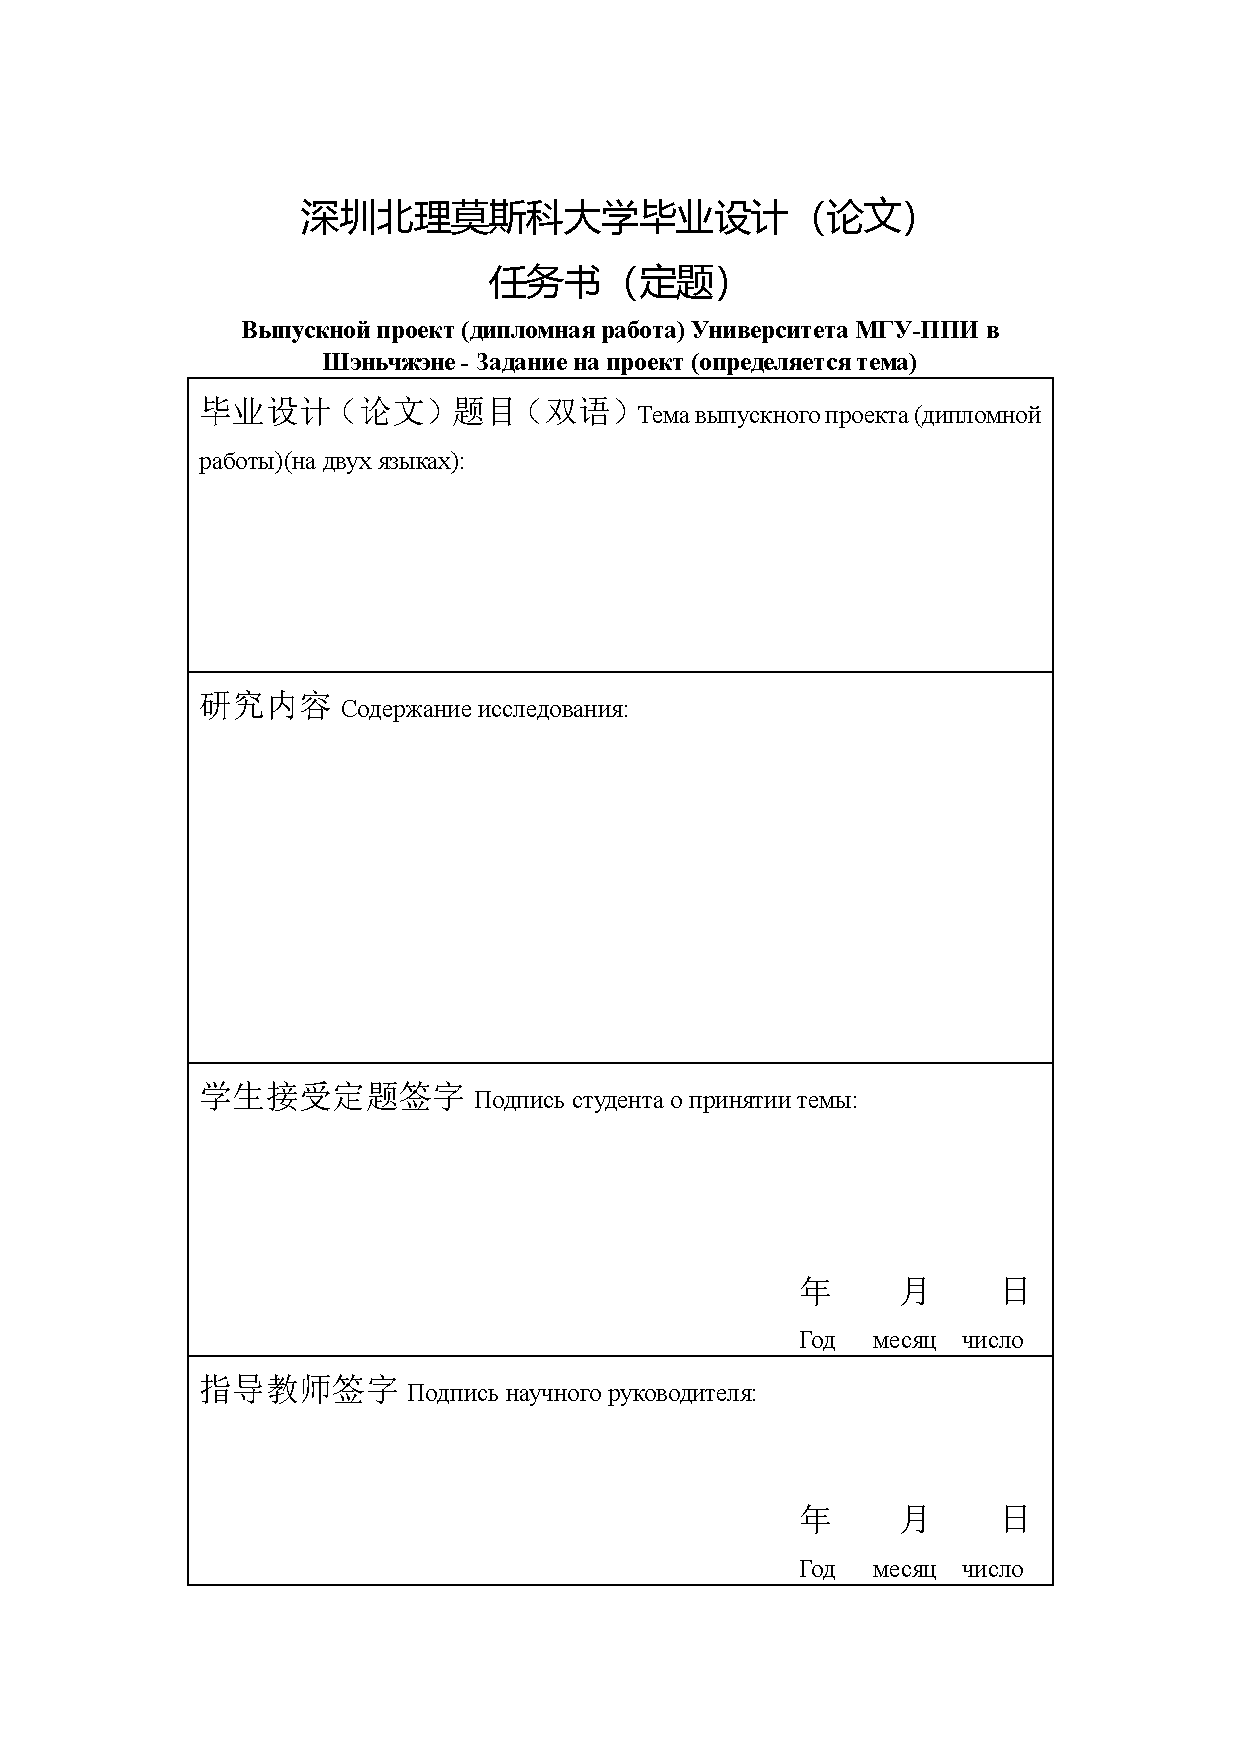
\includepdf[pages=1-5, pagecommand={\thispagestyle{fancy}}]{last.pdf}

\end{document}